\documentclass{article}
\usepackage{amsmath,graphicx}
\usepackage[margin=1in]{geometry}
\newcommand{\pderiv}[1]{\frac{\partial }{\partial #1}}
\newcommand{\ppderiv}[2]{\frac{\partial #1}{\partial #2}}
\newcommand{\del}{\mathbf{\nabla}}
\begin{document}

\section{Godunov Method}
We start with the hyperbolic equations of motion written in vector form,
\begin{equation}
    \partial_t \mathbf{U} + \mathbf{\nabla} \cdot \mathbf{F} = \mathbf{S}
\end{equation}
We integrate this over a cell with volume $V$, and use the divergence theorem to get the integral equations of motion,
\begin{equation}
    \frac{d }{d t} \frac{1}{V} \int dV \, \mathbf{U} + \frac{1}{V} \left( \mathbf{F}^+ - \mathbf{F}^- \right)= \frac{1}{V} \int dV \, \mathbf{S} 
\end{equation}
Define the volume averaged quantities as $\bar{\mathbf{U}} = \frac{1}{V} \int dV \, \mathbf{U}$, so that now,
\begin{equation}
    \frac{d }{d t} \bar{\mathbf{U}} + \frac{1}{V} \left( \mathbf{F}^+ - \mathbf{F}^- \right) = \bar{\mathbf{S}} 
\end{equation}
Now integrate in time from $t=0$ to $t=\Delta t$,
\begin{equation}
    \bar{\mathbf{U}}(\Delta t) - \bar{\mathbf{U}} + \frac{1}{V} \int dt \, \left( \mathbf{F}^+ - \mathbf{F}^- \right) = \int dt \, \bar{\mathbf{S}} 
\end{equation}
Up until this point we haven't made any approximations. The trick now is to evaluate the time-averaged boundary fluxes and source terms. We would also like to retain at least second order accuracy in time and space. To do this we'll use a MUSCLE-Hancock scheme with slope limiters and an approximate Riemann solver. 
\section{MUSCLE-Hancock Scheme}
This summary is taken from Toro p.557.
\begin{enumerate}
    \item Set boundary conditions
    \item Set timestep based on CFL condition.
        \begin{equation}
            \Delta t = C_{cfl} \frac{\Delta x}{S_\text{max}}
        \end{equation}
        where $S_\text{max}$ is the maximum wave speed. This is typically the faster of advection, sound speeds, viscous speeds, etc. 
    \item Data reconstruction and boundary extrapolated values.
        Use the primitive equation,
        \begin{equation}
            \partial_t \mathbf{W} + \mathbf{A}(\mathbf{W}) \partial_x \mathbf{W} = 0
        \end{equation}
        To evolve the boundary extrapolated values half a timestep, 
        \begin{eqnarray}
            \mathbf{W}_L &=& \mathbf{W}_i^n + \frac{1}{2} \left[ \mathbf{I} - \frac{\Delta t}{\Delta x} \mathbf{A}(\mathbf{W}_i^n) \right] \Delta _i , \\
            \mathbf{W}_R &=& \mathbf{W}_{i+1}^n - \frac{1}{2} \left[ \mathbf{I} + \frac{\Delta t}{\Delta x} \mathbf{A}(\mathbf{W}_{i+1}^n) \right] \Delta _{i+1} ,
        \end{eqnarray}
        where $\Delta_i$ are the slopes of the primitive variables to be determined below. 
    \item Solution of Riemann problem at each interface. 
        The Riemann problem uses $\mathbf{W}^{L,R}$ to determine $\mathbf{W}_{i+1/2,j}(x/t)$ in the $x$ direction. The interface fluxes are then,
        \begin{equation}
            \mathbf{F}_{i+1/2,j} = \mathbf{F}\left(\mathbf{W}_{i+1/2,j} (0) \right)
            \qquad 
            \mathbf{G}_{i,j+1/2} = \mathbf{G}\left(\mathbf{W}_{i,j+1/2} (0) \right)
        \end{equation}
        IF your cell is moving with some speed $\mathbf{w} = (w_x, w_y)$ (e.g if you have a Lagrangian mesh) then you would evaluate the fluxes at $x/t = w_x$ and $y/t = w_y$ rather than $x/t  = y/t = 0$.
\end{enumerate}

\subsection{Slopes and Slope-Limiters}
The slopes are,
\begin{equation}
    \Delta_i = \frac{1}{2} (1 + w) \Delta_{i-1/2} + \frac{1}{2} ( 1 - w) \Delta_{i+1/2} 
    \qquad
    \Delta_{i+1/2} = \mathbf{U}_{i+1}^n - \mathbf{U}_i^n
\end{equation}
The simplest limiter to use is the MINBEE/SUBERBEE limiter,
\begin{equation}
\Delta_i = 
\begin{cases}
 \text{max}\left[ 0 , \text{min}(\beta \Delta_{i-1/2}, \Delta_{i+1/2}), \text{min}(\Delta_{i-1/2}, \beta \Delta_{i+1/2}) \right],  & \Delta_{i+1/2} > 0 , \\
 \text{min}\left[ 0 , \text{max}(\beta \Delta_{i-1/2}, \Delta_{i+1/2}), \text{max}(\Delta_{i-1/2}, \beta \Delta_{i+1/2}) \right],  & \Delta_{i+1/2} < 0 
\end{cases}
\end{equation}
where $\beta=1,2$ correspond to the MINBEE and SUPERBEE limiters.


\section{HLLC Riemann Solver}

The HLLC solver puts the contact wave back into the HLL solver. 

\begin{enumerate}
\item Get wave speeds $S_L$, $S_\star$, $S_R$.
\item Construct $\mathbf{U}_L^\star$ and $\mathbf{U}_R^\star$.
\item Calculate $\mathbf{F}_*^{hllc}$.
\end{enumerate}



\subsection{Wave speeds}
Wave speeds are obtained from approximate simple Riemann solvers depending on the left-right states. These solvers are the primitive variable RS (PVRS), the two-rarefaction RS (TRRS), and the two-shock RS (TSRS). If the pressure jump at the interface is less than a user specified ratio (typically, $p_{max}/p_{pmin} < 2$) then the flow is smooth and the PVRS is used to estimate $p_\star$ and $u_\star$. If the pressure jump is larger than this ratio, there is likely either a shock or a rarefaction present. If the interface pressure, $p_\star$, given from the PVRS is less than $p_{min}$, then the rarefaction solver, TRRS, is used, else the shock solver, TSRS, is used. 

The estimates for the three approximate solvers for the pressure and velocity are,

\begin{equation}
p_{pvrs} = \frac{1}{2} ( p_L + p_R) - \frac{1}{2} ( u_R - u_L) C
\end{equation}
\begin{equation}
u_{pvrs} = \frac{1}{2} (u_L + u_R) - \frac{1}{2} \frac{p_R - p_L}{C}
\end{equation}
\begin{equation}
C = \frac{\rho_L + \rho_R}{2} \frac{a_L + a_R}{2}
\end{equation}

\begin{equation}
p_{trrs} = \left[ \frac{a_L+a_R - \frac{\gamma -1}{2} ( u_R - u_L)}{a_L/p_L^z + a_r/p_R^z}\right]^z
\end{equation}
\begin{equation}
u_{trrs} = \frac{P_{LR} u_L/a_L + u_R/a_R + \frac{2(P_{LR}-1)}{\gamma -1}}{P_{LR}/a_L + 1/a_R}
\end{equation}
\begin{equation}
z = \frac{\gamma -1}{2 \gamma} \qquad P_{LR} = \left( \frac{p_L}{p_R} \right)^z
\end{equation}
\begin{equation}
p_{tsrs} = \frac{g_L(p_0) p_L + g_R(p_0) p_R - (u_R - u_L)}{g_L(p_0) + g_r(p_0)}
\end{equation}
\begin{equation}
u_{tsrs} = \frac{1}{2} (u_L + u_R) + \frac{1}{2}\left[ (p_{tsrs}-p_R) g_R(p_0) - (p_{tsrs} - p_L) g_L(p_0) \right]
\end{equation}
\begin{equation}
g_K (p) =\sqrt{\frac{A_K}{p + B_K}} \qquad p_0 = max(0,p_{pvrs})
\end{equation}
\begin{equation}
A_K =  \frac{2}{\rho_K ( \gamma + 1 ) } \qquad B_K = \left( \frac{\gamma -1}{\gamma + 1} \right) p_K
\end{equation}

The estimates for the interface pressure and velocity are then,

\begin{equation}
p_\star,u_\star = 
\begin{cases}
p_{pvrs},u_{pvrs} & \frac{p_{max}}{p_{min}} < 2 \\
p_{trrs}, u_{trrs} & \frac{p_{max}}{p_{min}} > 2 \, \text{and} \, p_{pvrs} < p_{max} \\ 
p_{tsrs}, u_{tsrs} & \frac{p_{max}}{p_{min}} > 2 \, \text{and} \, p_{pvrs} > p_{max} \\ 
\end{cases}
\end{equation}

Now that we have $p_\star$ and $u_\star$ we can calculate the minimum, maxmimum and intermediate wave speeds as,

\begin{equation}
S_L = u_L - a_L q_L
\end{equation}
\begin{equation}
S_L = u_R + a_R q_R
\end{equation}
\begin{equation}
S_\star = \frac{ p_R - p_L + \rho_L u_L (S_L - u_L) - \rho_R u_R (S_R - u_R)}{\rho_L (S_L - u_L) - \rho_R (S_R - u_R)}
\end{equation}
\begin{equation}
q_K = 
\begin{cases}
1 & p_\star \le p_K \\
\sqrt{ 1 + \frac{\gamma +1}{2 \gamma}\left( \frac{p_\star}{p_K} - 1 \right)} & p_\star > p_K
\end{cases}
\end{equation}

\subsection{Star region}
Now that we have the wave speeds the conservative left and right states in the starred region are,

\begin{equation}
\mathbf{U}_K^\star = \rho_K \left( \frac{ S_K - u_K}{S_K - S_\star} \right) \left[
\begin{matrix}
1 \\ 
S_\star \\
v_K \\
w_K \\
\frac{E_K}{\rho_K} + (S_\star - u_K) \left[ S_\star  + \frac{p_K}{\rho_K(S_K-u_K)} \right]
\end{matrix}
\right]
\end{equation}
Additionally, any passive scalar is advected in the same way as the tangential velocities, i.e
\begin{equation}
(\rho q)_\star^K = \rho_K \left( \frac{S_K - u_K}{S_K - S_\star} \right) q_k
\end{equation}


\subsection{Final flux}

Finally, the HLLC flux is,

\begin{equation}
\mathbf{F}_{i+1/2}^{hllc} = 
\begin{cases}
\mathbf{F}_L & 0 \le S_L \\
\mathbf{F}_L + S_L(\mathbf{U}_\star^L - \mathbf{U}_L) & S_L \le 0 \le S_\star \\
\mathbf{F}_R + S_R(\mathbf{U}_\star^R - \mathbf{U}_R) & S_\star \le 0 \le S_R \\
\mathbf{F}_R & 0 \ge S_R \\
\end{cases}
\end{equation}

\section{Equations of motion for orthogonal coordinate system}
For an orthogonal coordinate system $(x_i,x_j,x_k)$ with diagonal metric $g_{ij} = h_ i^2 \delta_{ij}$, scale factors $h_i$, coordinate vectors  $\mathbf{e}_i = h_i \hat{\mathbf{e}}_i $, the volume element is $\Delta V = dv \Delta x_1 \Delta x_2 \Delta x_3$ where $dv \equiv h_1 h_2 h_3$, the surface area elements are, $\Delta S_i = ds_i \Delta x_j \Delta x_k$, and where $ds_i \equiv dv / h_i$, where $i,j,k$ are cyclic indices (so no Einstein summation)

The gradient of a scalar, $\Phi$ is,
\begin{equation}
\del \Phi = \frac{1}{h_i} \ppderiv{\Phi}{x_i} \hat{\mathbf{x}}_i  + \frac{1}{h_j} \ppderiv{\Phi}{x_j} \hat{\mathbf{x}}_j + \frac{1}{h_k} \ppderiv{\Phi}{x_k} \hat{\mathbf{x}}_k 
\end{equation}
The Laplacian is,
\begin{equation}
dv \nabla^2 \Phi = \pderiv{x_i}\left( \frac{ds_i}{h_i} \ppderiv{\Phi}{x_i} \right) + \pderiv{x_j}\left( \frac{ds_j}{h_j} \ppderiv{\Phi}{x_j}\right)  + \pderiv{x_k}\left( \frac{ds_k}{h_k}\ppderiv{\Phi}{x_k}\right) 
\end{equation}
The divergence of a vector $\mathbf{v}$ is,
\begin{equation}
d v (\del \cdot \mathbf{v}) = \pderiv{x_i} \left( ds_i v_i \right) +\pderiv{x_j} \left( ds_j v_j \right) +\pderiv{x_k} \left( ds_k v_k \right)  
\end{equation}
The divergence of a vector $\mathbf{v}$ is,
\begin{equation}
ds_i \left(\del \times \mathbf{v} \right) \cdot \hat{\mathbf{x}}_i = \pderiv{x_j} \left( h_k v_k \right) - \pderiv{x_k} \left( h_j v_j \right)
\end{equation}
The divergence of a tensor, $\mathbf{T}$, is, 
\begin{align} 
d v \left(\del \cdot \mathbf{T} \right) \cdot \hat{\mathbf{x}}_i &= \pderiv{x_i} \left( ds_i T_{ii} \right)  +  \pderiv{x_j} \left( ds_j T_{ij} \right) +  \pderiv{x_k} \left( ds_k T_{ik} \right)  \nonumber \\
&+  T_{ij} ds_j  \frac{1}{h_i} \ppderiv{h_i}{x_j}+ T_{ki} ds_k \frac{1}{h_i} \ppderiv{h_i}{x_k} - T_{jj} ds_i \frac{1}{h_j} \ppderiv{h_j}{x_i} - T_{kk} ds_i \frac{1}{h_k} \ppderiv{h_k}{x_i}
\end{align}

We can simplify this further for symmetric tensors, $\mathbf{T} = \mathbf{S}$, and diagonal tensors, $T_{ij} = P \delta_{i,j}$
\begin{align}
dv \left(\del \cdot \mathbf{S} \right)\cdot \hat{\mathbf{x}}_i &= \pderiv{x_i} \left( ds_i S_{ii} \right)  +  \frac{1}{h_i}\pderiv{x_j} \left( h_i ds_j S_{ij} \right) +  \frac{1}{h_i} \pderiv{x_k} \left( h_i ds_k S_{ik} \right) - S_{jj} h_k \ppderiv{h_j}{x_i} - S_{kk} h_j  \ppderiv{h_k}{x_i}  \\
dv \left(\del \cdot \mathbf{P} \right)\cdot \hat{\mathbf{x}}_i  &= \pderiv{x_i} \left( ds_i P \right)   -  P \ppderiv{(ds_i)}{x_i}  
\end{align}
where again the indices $ijk$ are not summed over but instead are cyclic $i \rightarrow j \rightarrow k$.
The point of this form is that if you have a coordinate system where the scale factors only depend on one of the coordinates, then then the non divergence terms for a symmetric tensor will be zero in two of the directions. This is useful for conservation properties. 
The diagonal tensor non-divergence term evaluates to $-P$.



For the Euler equations we have,

\begin{align}
dv \ppderiv{(\rho v_i)}{t} &+ \pderiv{x_i} \left( ds_i (\rho v_i^2 + P) \right) + \frac{1}{h_i} \pderiv{x_j} \left(h_i ds_j  \rho v_i v_j \right) + \frac{1}{h_i} \pderiv{x_k} \left(h_i ds_k \rho v_i v_k \right)  \nonumber \\ 
&- \rho v_j^2  h_k \ppderiv{h_j}{x_i} - \rho v_k^2 h_j \ppderiv{h_k}{x_i} - P \ppderiv{(ds_i)}{x_i} \\ 
dv \ppderiv{\rho}{t} &+ \pderiv{x_i} \left( ds_i \rho v_i \right) +\pderiv{x_j} \left( ds_j \rho v_j \right) +\pderiv{x_k} \left( ds_k \rho v_k \right)  = 0 \\
dv \ppderiv{E}{t} &+ \pderiv{x_i} \left( ds_i (E + P) v_i \right) +\pderiv{x_j} \left( ds_j (E + P)  v_j \right) +\pderiv{x_k} \left( ds_k (E + P) v_k \right)  = 0 \\
\end{align}
where $E = P/(\gamma-1) + \rho v^2/2$.

All fluxes are then weighted by the surface area of the cell's face in the update equation,
\begin{equation}
\frac{d}{dt} \frac{1}{V} \int dV Q  + \frac{1}{V} \left( S^+ F^+ - S^- F^- \right) = \frac{1}{V} \int dV S
\end{equation}

\subsubsection{Cartsian}
In cartesian all scale factors are unity, $h = 1, ds = 1, dv=1$.
\begin{align}
\ppderiv{(\rho v_i)}{t} &+ \pderiv{x_i} \left(\rho v_i^2 + P \right) +  \pderiv{x_j} \left( \rho v_i v_j \right) + \pderiv{x_k} \left( \rho v_i v_k \right)  = 0 \\ 
 \ppderiv{\rho}{t} &+ \pderiv{x_i} \left( \rho v_i \right) +\pderiv{x_j} \left( \rho v_j \right) +\pderiv{x_k} \left( \rho v_k \right)  = 0
 \end{align}
\subsubsection{Cylindrical}
In cylindrical $(r,\phi,z)$, the only non-unity scale factors are $h_\phi = ds_r = ds_z = dv = r$
\begin{align}
r \ppderiv{(\rho v_r)}{t} &+ \pderiv{r} \left( r \rho v_r^2 + r P \right)  + \pderiv{\phi} \left(  \rho v_r v_\phi \right) + \pderiv{z} \left(r  \rho v_r v_z \right)  - \rho v_\phi^2 - P = 0 \\
r \ppderiv{(\rho v_\phi)}{t} &+ \frac{1}{r} \pderiv{r} \left( r^2 \rho v_r v_\phi \right) + \pderiv{\phi} \left(  \rho v_\phi^2 + P \right) + \frac{1}{r} \pderiv{z} \left(r^2 \rho v_\phi v_z \right)  = 0 \\
r \ppderiv{(\rho v_z)}{t} &+ \pderiv{r} \left( r \rho v_r v_z \right) + \pderiv{\phi} \left( \rho v_\phi v_z \right) + \pderiv{z} \left( r \rho v_z^2 + r P \right) = 0 \\
r \ppderiv{\rho}{t} &+ \pderiv{r} \left( r \rho v_r \right) + \pderiv{\phi} \left(\rho v_\phi \right) + \pderiv{z} \left(r  \rho v_z \right)  
\end{align}
\subsubsection{Spherical}
In spherical $(r,\theta,\phi)$, the non-unity scale factors are, $h_\phi =r \sin \theta, h_\theta = r, ds_r =dv= r^2 \sin \theta, ds_\phi = r,$ and $ds_\theta = r \sin\theta$
\begin{align}
r^2 \sin \theta \ppderiv{(\rho v_r)}{t} &+ \pderiv{r} \left( r^2 \sin \theta (\rho v_r^2 + P) \right) + \pderiv{\theta} \left( r \sin \theta \rho v_r v_\theta \right) + \pderiv{\phi} \left( r \rho v_r v_\phi \right) \nonumber \\
&- r \rho v_\theta^2 - r \sin \theta \rho v_\phi^2  - 2 P r \sin \theta = 0 \\
r^2 \sin \theta \ppderiv{(\rho v_\theta)}{t} &+ \pderiv{r} \left( r^3 \sin \theta \rho v_r v_\theta \right) + \pderiv{\theta} \left( r \sin \theta ( \rho v_\theta^2 + P) \right) + \frac{1}{r} \pderiv{\phi} \left( r^2 \rho v_\phi v_\theta \right) \nonumber \\ 
&- r \cos \theta \rho v_\phi^2 - P r \cos{\theta} = 0 \\
r^2 \sin \theta \ppderiv{(\rho v_\phi)}{t} &+ \frac{1}{r \sin \theta} \pderiv{r} \left( r^3 \sin^2 \theta \rho v_r v_\phi \right) + \frac{1}{r \sin \theta} \pderiv{\theta} \left( r^2 \sin^2 \theta \rho v_\theta v_\phi \right) + \pderiv{\phi} \left( r \rho v_\phi^2 + r P \right) = 0 \\
r^2 \sin \theta \ppderiv{\rho}{t} &+ \pderiv{r} \left( r^2 \sin \theta \rho v_r \right) + \pderiv{\phi} \left(r \rho v_\phi \right) + \pderiv{\theta} \left(r \sin \theta  \rho v_\theta \right)   = 0
\end{align}


\section{Non-orthogonal}
In a non-orthogonal coordinate system with metric $g_{ij}$, the fluid equations are,
\begin{align}
\ppderiv{\rho}{t} + \del_i \left( \rho V^i \right) = 0 \\
\pderiv{t} (\rho V^j)  + \del_i \left(\rho V^i V^j  \right) = -\del_i P
\end{align}

To mirror what we did for the orthogonal coordinate systems we can write this in a mixed basis,
\begin{align}
\pderiv{t} (\sqrt{g} \rho ) + \pderiv{x^i} \left( \sqrt{g} \rho V^i\right) = 0 \\
\pderiv{t} ( \sqrt{g} \rho V_j)  + \pderiv{x^i} \left( \sqrt{g} T_j^i  \right) = -\sqrt{g} \pderiv{x^i} P + \sqrt{g} T_k^j \Gamma_{ij}^k
\end{align}
where $\sqrt{g} = {\rm det}(g)$,  $T^{ij} = \rho V^i V^j$, and 
\begin{equation}
	T_j^i = g_{jk} T^{ki} = \rho g_{jk} V^k V^i = \rho V_j V^i = \rho V_j g^{ik} V_k
\end{equation}
Note that $V_i = g_{ij} V^j = v_i /h^i $ where $v_i$ is the physical velocity so that $T_j^i$ is,
\begin{equation}
T_j^i = \frac{\rho}{h^j h_k} v_j g^{ik} v_k 
\end{equation}
\begin{align}
\pderiv{t} (\sqrt{g} \rho ) &+ \pderiv{x^i} \left( \frac{\sqrt{g}}{h^k} \rho g^{ik} v_k \right) = 0 \\
\pderiv{t} ( \frac{\sqrt{g}}{h^j} \rho v_j)  &+ \pderiv{x^i} \left( \frac{\sqrt{g}}{h^j h_k} \rho v_j g^{ik} v_k \right) = - \sqrt{g}\pderiv{x^i} P + \frac{\sqrt{g}}{h^k h_j} \rho v_k  g^{j \ell} v_\ell \Gamma_{ij}^k 
\end{align}




\section{CTU}
\begin{enumerate}
\item For each direction in the problem
\begin{enumerate}
    \item Solve for left/right interface states, $U_L$ and $U_R$ for each cell
    \begin{enumerate}
    	\item This entails limiting the left and right slopes and evolving $U_{L,R}$ for $\Delta t/2$ using the fluxes, $F(U_{L,R})$. This can be PCM, PLM, PPM, WENO, etc., for first order, second order, third order, and higher order, respectively.
    \end{enumerate}
    \item Compute the fluxes at the interfaces by solving the Riemann problem $F(U_L,U_R)$.
\end{enumerate}
\item Using the fluxes in each direction, update $U_{L,R}$ in each direction by using the fluxes in the \emph{transverse} directions to evolve $U_{L,R}$ for $\Delta t/2$. 

\item Recompute the fluxes in each direction by solving the Riemann problem at the interfaces with the corrected $U_{L,R}$. 
\item Update the conserved variables in each cell using the corrected interface fluxes in each direction for a full $\Delta t$.
\end{enumerate}

\subsection{1D Timestepping algorithm} 
Let the conserved variables be $U = \left\{\rho, \rho v_x, \rho v_y, \rho v_z, E \right\}$, and the flux be $F = \left\{ \rho v_x, \rho v_x^2 + P, \rho v_x v_y, \rho v_x v_z, v_x (E + P) \right\}$ so that in 1D,
\begin{equation}
	\ppderiv{U}{t} +\ppderiv{F}{x} = 0
\end{equation}
Let $U_i^n$ represent the volume averaged conserved variables in cell $i$ at time $t_n$. 
To go from $U_i^n$ to $U_i^{n+1}$ at time $t_{n+1} = t_n + \Delta t$ we do the following,
\begin{enumerate}
	\item Reconstruct the values of $U_{i+1/2}$ from the gradient estimates of $U_{i}-U_{i-1}$ and $U_{i+1}-U_{i}$. This gives the quantities, $U_i^L$ and $U_i^R$ which are defined at the boundary between cell $i$ and cell $i+1$. 
	\item Evolve $U_i^L$ and $U_i^R$ for $\Delta t/2$ by the fluxes $F(U_i^L)$ and $F(U_i^R)$,
	\begin{align}
		U_i^{L,n+1/2} &= U_i^{L,n} - \frac{\Delta t}{2 \Delta x} \left( F(U_i^L) -F(U_{i-1}^R \right) \\
		U_{i-1}^{R,n+1/2} &= U_{i-1}^{R,n} - \frac{\Delta t}{2 \Delta x} \left( F(U_i^L) -F(U_{i-1}^R \right)
	\end{align}
	The index convention is that $U_i^{L,R}$ lie at the right interface of cell $i$, so at $i+1/2$. 
	\item Solve for the interface flux by solving the 1D Riemann problem $F_i = F(U_i^{L,n+1/2},U_i^{R,n+1/2})$. 
	\item Given the left and right fluxes, $F_{i-1}$ and $F_{i}$ update the volume averaged conserved variables, 
	\begin{equation}
		U_i^{n+1} = U_i^n - \frac{\Delta t}{\Delta x} \left(F_i - F_{i-1} \right)
	\end{equation}

\end{enumerate}
\subsection{1D Timestepping algorithm with potential source} 
With a time independent potential the equations of motion have a source term, 
\begin{equation}
	\ppderiv{U}{t} +\ppderiv{F}{x} = S
\end{equation}
where $S = \left\{0,-\rho \partial \Phi/ \partial x, -\rho \partial \Phi / \partial y , -\rho \partial \Phi/\partial z, -\rho v \cdot \del \Phi \right\}$
The Reconstruct-Evolve-Solve-Update algorithm given above is essentially the same, the only difference is including the source term in the Evolve and Update steps.
\begin{enumerate}
	\item Reconstruct the values of $U_{i+1/2}$ from the gradient estimates of $U_{i}-U_{i-1}$ and $U_{i+1}-U_{i}$. This gives the quantities, $U_i^L$ and $U_i^R$ which are defined at the boundary between cell $i$ and cell $i+1$. 
	\item Evolve $U_i^L$ and $U_i^R$ for $\Delta t/2$ by the fluxes $F(U_i^L)$ and $F(U_i^R)$,
	\begin{align}
		U_i^{L,n+1/2,*} &= U_i^{L,n} - \frac{\Delta t}{2 \Delta x} \left( F(U_i^L) -F(U_{i-1}^R \right)  \\
		U_{i-1}^{R,n+1/2,*} &= U_{i-1}^{R,n} - \frac{\Delta t}{2 \Delta x} \left( F(U_i^L) -F(U_{i-1}^R \right) \\
	\end{align}
	\item Evolve these interface states for $\Delta t /2$ using the source term. For the momenta, this is
	\begin{align}
		U_i^{L,n+1/2} &= U_i^{L,n+1/2,*} - \frac{\Delta t}{\Delta x} \rho_i^{L,n+1/2,*} \left(\Phi_{i+1/2}-\Phi_i\right) \\
		U_{i-1}^{R,n+1/2} &= U_{i-1}^{R,n+1/2,*}  - \frac{\Delta t}{\Delta x} \rho_{i-1}^{R,n+1/2,*}\left(\Phi_{i}-\Phi_{i-1/2}\right)
	\end{align}
	where $U$ for the 1D case is $\rho v_x$.
	Note that this is equivalent to updating the primitive velocity, $v_x$. 
	\item Solve for the interface flux by solving the 1D Riemann problem $F_i = F(U_i^{L,n+1/2},U_i^{R,n+1/2})$. 
	\item Compute the density at $\Delta t/2$ using the fluxes, $F_i$. 
	\begin{equation}
		\rho_i^{n+1/2} = \rho_i^n - \frac{\Delta t}{2 \Delta x} \left(F_i^\rho - F_{i-1}^\rho \right) 
	\end{equation}
	where $F^\rho = \rho v_x$ is the density component of the flux. 
	\item Given the left and right fluxes, $F_{i-1}$ and $F_{i}$, and $\rho_i^{n+1/2}$, update the volume averaged conserved variables. 
	For the momenta,
	\begin{equation}
		U_i^{n+1} = U_i^n - \frac{\Delta t}{\Delta x} \left(F_i - F_{i-1} \right) - \frac{\Delta t}{\Delta x} S_i
	\end{equation}
	where $S_i$ is zero for the density, 
	\begin{equation}
		\rho_i^{n+1/2} \left( \Phi_{i+1/2}-\Phi_{i-1/2} \right)
	\end{equation}
	for the momenta, and 
	\begin{equation}
		F_i^\rho \left(\Phi_{i+1/2}-\Phi_i\right) + F_{i-1}^\rho \left(\Phi_{i}-\Phi_{i-1/2}\right)
	\end{equation}
	for the energy. 


\end{enumerate}


\subsection{2D Timestepping algorithm } 
In 2D we have an additional flux in the $y$ direction, $G= \left\{ \rho v_y, \rho v_x v_y, \rho v_y^2 + P, \rho v_y v_z, v_y (E + P) \right\}$
\begin{equation}
	\ppderiv{U}{t} +\ppderiv{F}{x}  + \ppderiv{G}{y} = 0
\end{equation}
Let $U_{i,j}^n$ represent the volume averaged conserved variables in cell $(i,j)$ at time $t_n$.
The first steps are the same as the 1D algorithm, 
\begin{enumerate}
	\item Reconstruct-Evolve-Solve in $x$ direction to obtain $U_{i,j}^{L,R,n}$ and $F_{i,j}^n$.
	\item Reconstruct-Evolve-Solve in $y$ direction to obtain $U_{i,j}^{L,R,n}$ and $G_{i,j}^n$.  
	\item Evolve the left and right states using the \emph{transverse} fluxes, 
	\begin{align}
		U_{i+1/2,j}^{L,n+1/2} &= U_{i+1/2,j}^{L,n} - \frac{\Delta t}{2 \Delta y} \left( G_{i,j}^n - G_{i,j-1}^n \right) \\
		U_{i+1/2,j}^{R,n+1/2} &= U_{i+1/2,j}^{R,n} - \frac{\Delta t}{2 \Delta y} \left( G_{i+1,j}^n - G_{i+1,j-1}^n \right) \\
		U_{i,j+1/2}^{L,n+1/2} &= U_{i,j+1/2}^{L,n} - \frac{\Delta t}{2 \Delta x} \left( F_{i,j}^n - F_{i-1,j}^n \right) \\
		U_{i,j+1/2}^{R,n+1/2} &= U_{i,j+1/2}^{R,n} - \frac{\Delta t}{2 \Delta x} \left( F_{i,j+1}^n - F_{i-1,j+1}^n \right)
	\end{align}
	\item Solve the Riemann problem for the corrected interface fluxes, $F_{i,j}^{n+1/2} = F(U_{i+1/2,j}^{L,n+1/2}, U_{i+1/2,j}^{R,n+1/2})$ and $G_{i,j}^{n+1/2} = F(U_{i,j+1/2}^{L,n+1/2},U_{i,j+1/2}^{R,n+1/2})$. 

	\item Given the interface fluxes, update the volume averaged conserved variables, 
	\begin{equation}
		U_i^{n+1} = U_i^n - \frac{\Delta t}{\Delta x} \left(F_{i,j}^{n+1/2} - F_{i-1,j}^{n+1/2} \right) - \frac{\Delta t}{\Delta y} \left(G_{i,j}^{n+1/2} - G_{i,j-1}^{n+1/2} \right)
	\end{equation}
\begin{figure}
\centering
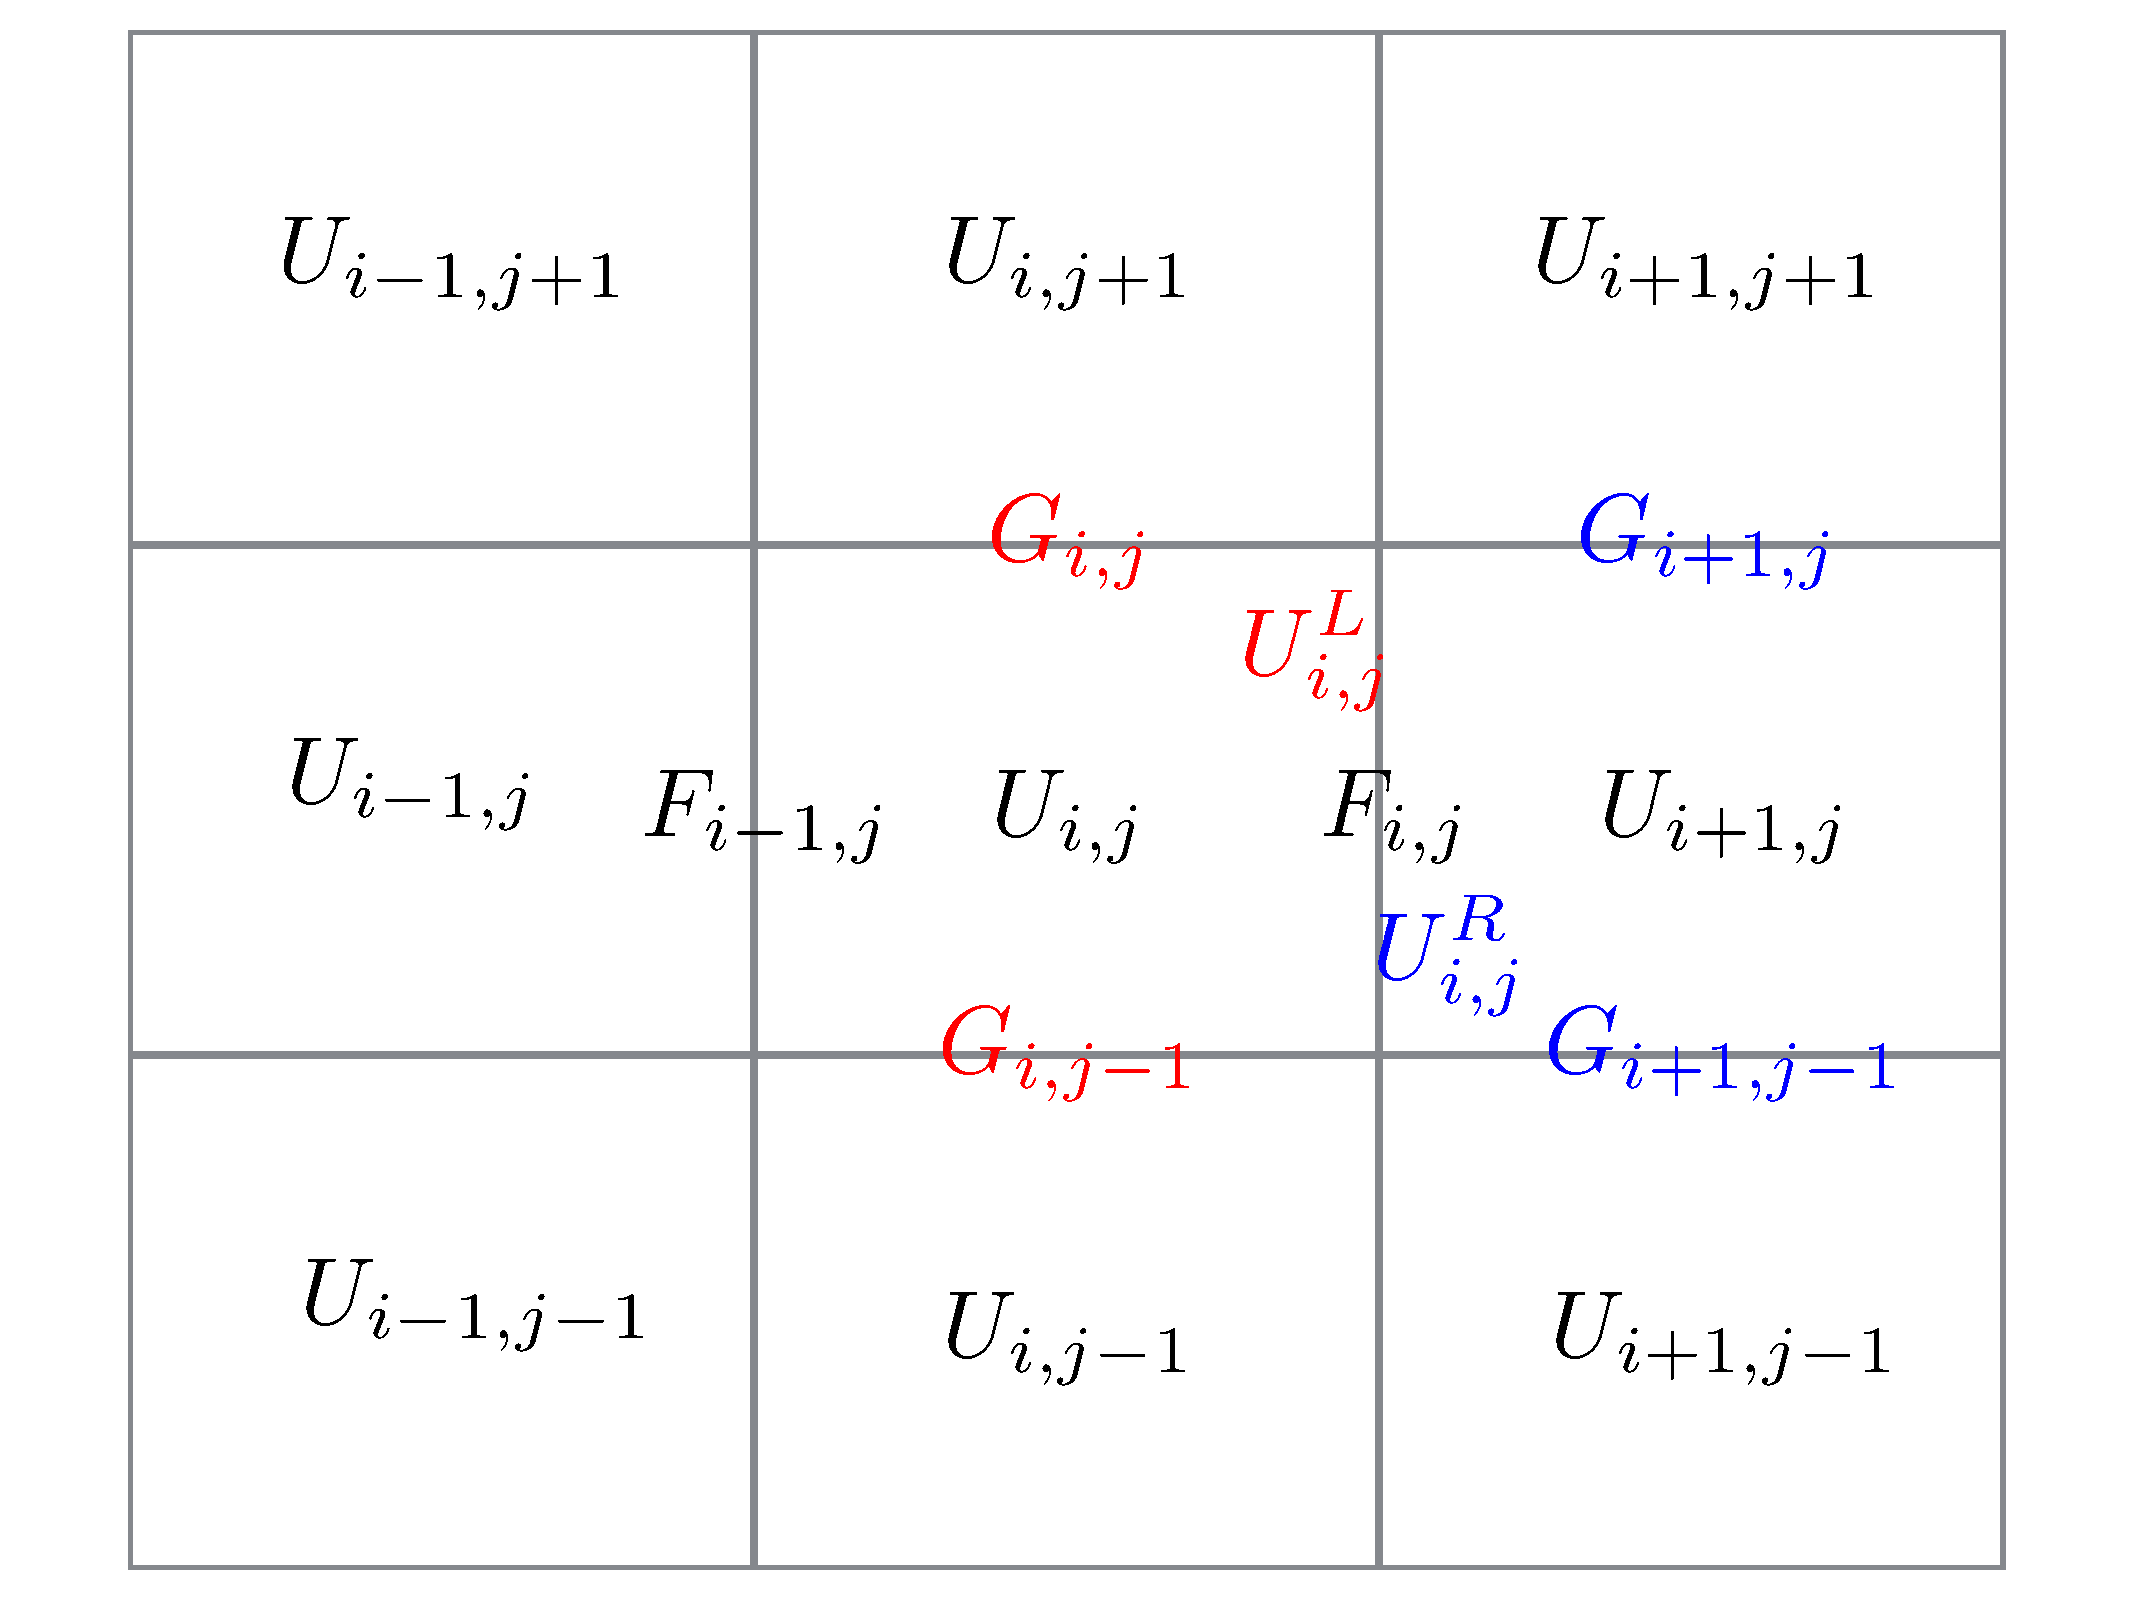
\includegraphics[width=.8\textwidth]{2d_transverse}
\end{figure}
\end{enumerate}

\subsection{2D Timestepping algorithm with Potential} 
Adding the source term changes the equations of motion to,
\begin{equation}
	\ppderiv{U}{t} +\ppderiv{F}{x}  + \ppderiv{G}{y} = S
\end{equation}
with  $S = \left\{0,-\rho \partial \Phi/ \partial x, -\rho \partial \Phi / \partial y , -\rho \partial \Phi/\partial z, -\rho v \cdot \del \Phi \right\}$.
The full algorithm is,
\begin{enumerate}
	\item Reconstruct-Evolve-Solve in $x$ direction to obtain $U_{i,j}^{L,R,n}$ and $F_{i,j}^n$ (see 1D with source above).
	\item Reconstruct-Evolve-Solve in $y$ direction to obtain $U_{i,j}^{L,R,n}$ and $G_{i,j}^n$.  
	\item Evolve the left and right states using the \emph{transverse} fluxes, 
	\begin{align}
		U_{i,j}^{L,n+1/2,*} &= U_{i,j}^{L,n} - \frac{\Delta t}{2 \Delta y} \left( G_{i,j}^n - G_{i,j-1}^n \right) \\
		U_{i-1,j}^{R,n+1/2,*} &= U_{i-1,j}^{R,n} - \frac{\Delta t}{2 \Delta y} \left( G_{i+1,j}^n - G_{i+1,j-1}^n \right) \\
		U_{i,j}^{D,n+1/2,*} &= U_{i,j}^{D,n} - \frac{\Delta t}{2 \Delta x} \left( F_{i,j}^n - F_{i-1,j}^n \right) \\
		U_{i,j-1}^{U,n+1/2,*} &= U_{i,j-1}^{U,n} - \frac{\Delta t}{2 \Delta x} \left( F_{i,j+1}^n - F_{i-1,j+1}^n \right)
	\end{align}
	where $L,R,U,D$ correspond to left,right,up,down. 
	\item Evolve the left and right states using the transverse source terms, 
	\begin{align}
		U_{i,j}^{L,n+1/2} &= U_{i,j}^{L,n+1/2,*} - \frac{\Delta t}{\Delta y} \rho_{i,j}^{L,n+1/2,*} \left(\Phi_{i,j+1/2}-\Phi_{i,j}\right) \\
		U_{i-1,j}^{R,n+1/2} &= U_{i-1,j}^{R,n+1/2,*}  - \frac{\Delta t}{\Delta y} \rho_{i-1,j}^{R,n+1/2,*}\left(\Phi_{i,j}-\Phi_{i,j-1/2}\right) \\
		U_{i,j}^{D,n+1/2} &= U_{i,j}^{D,n+1/2,*} - \frac{\Delta t}{\Delta x} \rho_{i,j}^{D,n+1/2,*} \left(\Phi_{i+1/2,j}-\Phi_{i,j}\right) \\
		U_{i,j-1}^{U,n+1/2} &= U_{i,j-1}^{U,n+1/2,*}  - \frac{\Delta t}{\Delta x} \rho_{i,j-1}^{U,n+1/2,*}\left(\Phi_{i,j}-\Phi_{i-1/2,j}\right) \\
	\end{align}
	\item Solve the Riemann problem for the corrected interface fluxes, $F_{i,j}^{n+1/2} = F(U_{i,j}^{L,n+1/2}, U_{i,j}^{R,n+1/2})$ and $G_{i,j}^{n+1/2} = F(U_{i,j}^{U,n+1/2},U_{i,j}^{D,n+1/2})$. 
	\item Calculate $\rho_i^{n+1/2}$ with the fluxes,
	\begin{equation}
		\rho_i^{n+1/2} = \rho_i^n - \frac{\Delta t}{2 \Delta x} \left(F_{i,j}^{\rho,n+1/2} - F_{i-1,j}^{\rho,n+1/2} \right)  - \frac{\Delta t}{2 \Delta y} \left(G_{i,j}^{\rho,n+1/2} - G_{i,j-1}^{\rho,n+1/2} \right) 
	\end{equation}

	\item Given the interface fluxes and $\rho_i^{n+1/2}$ update the volume averaged conserved variables, 
	\begin{equation}
		U_i^{n+1} = U_i^n - \frac{\Delta t}{\Delta x} \left(F_{i,j}^{n+1/2} - F_{i-1,j}^{n+1/2} \right) - \frac{\Delta t}{\Delta y} \left(G_{i,j}^{n+1/2} - G_{i,j-1}^{n+1/2} \right) - \frac{\Delta t}{\Delta x} S_{i,x} - \frac{\Delta t}{\Delta y} S_{i,j,y}
	\end{equation}
	where $S_i$ is zero for the density, 
	\begin{equation}
		S_{i,j,x} = \rho_i^{n+1/2} \left( \Phi_{i+1/2,j}-\Phi_{i-1/2,j} \right) \qquad S_{i,j,y} = \rho_i^{n+1/2} \left( \Phi_{i,j+1/2}-\Phi_{i,j-1/2} \right)
	\end{equation}
	for the momenta, and
	\begin{align}
		S_{i,j,x} &= F_{i,j}^\rho \left(\Phi_{i+1/2,j}-\Phi_{i,j}\right) + F_{i-1,j}^\rho \left(\Phi_{i,j}-\Phi_{i-1/2,j}\right) \\
		S_{i,j,y} &= G_{i,j}^\rho \left(\Phi_{i,j+1/2}-\Phi_{i,j}\right) + G_{i,j-1}^\rho \left(\Phi_{i,j}-\Phi_{i,j-1/2}\right)
	\end{align}
	for the energy.

\end{enumerate}

\end{document}
